\documentclass[tikz,10pt,border=2mm]{standalone}
\usepackage{mathpazo,zi4,calligra,xcolor,structmech,siunitx}
\usetikzlibrary{backgrounds}
\definecolor{0066CC}{RGB}{0,102,204}
\definecolor{CC0066}{RGB}{204,0,102}
\definecolor{00CC66}{RGB}{0,204,102}
\definecolor{CC6600}{RGB}{204,102,0}
\definecolor{DDDDDD}{RGB}{204,204,204}
\begin{document}
\scriptsize
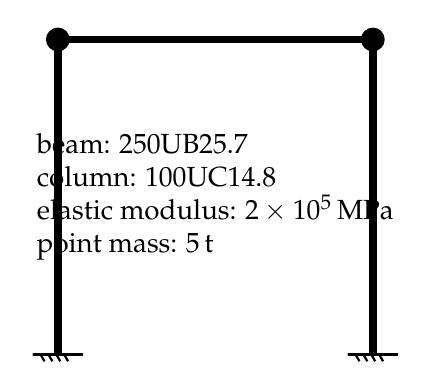
\begin{tikzpicture}
\setstructmech{linewidth=.8pt}
\def\s{4}
\FixedSupport{0,0}{.8}
\FixedSupport{\s,0}{.8}
\draw[line width=1mm](0,0)--(0,\s)node[draw,circle,inner sep=0,minimum size=2mm,fill=black]{}--(\s,\s)node[draw,circle,inner sep=0,minimum size=2mm,fill=black]{}--(\s,0);
\node[align=left]at(\s/2,\s/2){beam: 250UB25.7\\column: 100UC14.8\\elastic modulus: \SI{2E5}{\mega\pascal}\\point mass: \SI{5}{\tonne}};
\end{tikzpicture}
\end{document}